%!TEX root = ../09-Photoelectric-Effect.tex
\chapter{Photoelectric Effect}


\section{Open Circuit Voltage}%3.1


\section{Stopping Voltage}%3.2 and 3.5


\section{Photocurrent}%3.3 and 3.4

The current flowing through the photoelectric cell is measured while the voltage across its terminals is held at constant levels ranging from \SIrange{-3}{6}{\volt}.
The experiment is repeated with a neutral density filter in front of the mercury lamp.

\textbf{Setup}\\
A schematic of the setup is shown in \autoref{sch:photocurrent}.
A shunt resistor of $R_\text{shunt} = \SI{100}{\mega\ohm}$ is used, the output voltage $U_\text{out}$ is buffered by the electrometer to minimize the additional load.
The voltage $U_\text{g}$ is generated by a potentiometer connected across a \SI{9}{\volt} battery, it is read from a panel meter.

The actual stopping potential is $U_\text{s} = U_\text{g} - U_\text{out}$, the photocurrent is calculated as $I_\text{ph} = \frac{U_\text{out}}{R_\text{shunt}}$.

\textbf{Evaluation}\\
The measured values for the series with and without filter are plotted in \autoref{plt:photocurrent}.
There is no measurable reverse current, so measurements for $U_\text{g} < \SI{-1.6}{\volt}$ are omitted.

Both curves start around \SI{-1.5}{\volt} looking similar to the characteristic diode curve.
For higher stopping potentials, the current approaches the saturation current.

To approximate the saturation current, a logistic curve is fitted to the data as it is the most accurate model tested:
\begin{equation*}
	I_\text{ph}(U_\text{s}) = \frac{I_\text{sat}}{1 + \mathrm{e}^{-b (U_\text{s} - U_0)}},
\end{equation*}
resulting in
\begin{gather*}
	I_\text{sat} = \SI{37}{\nA}, \quad U_0 = \SI{1.64}{\volt}, \quad b = \SI{1.28}{\per\volt} \tag{no filter}\\
	I_\text{sat} = \SI{23}{\nA}, \quad U_0 = \SI{1.86}{\volt}, \quad b = \SI{1.15}{\per\volt}. \tag{filter}\\
\end{gather*}

The saturation current is proportional to the filter's transmittance, so the transmittance can be calculated as
\begin{equation*}
	T = \frac{I_\text{sat, filter}}{I_\text{sat, \#nofilter (todo)}} = \num{0.62}.
\end{equation*}

\begin{figure}[tbp]
	\centering
	\includegraphics[width=.4\textwidth]{img/photocurrent.pdf}
	\caption[Setup for measuring Photocurrent]{\textbf{Setup for measuring Photocurrent}}
	\label{sch:photocurrent}
\end{figure}

\begin{figure}[tbp]
	\centering
	\includegraphics[width=.8\textwidth]{data/plots/photocurrent.pdf}
	\caption[Photocurrent versus Stopping Potential]{\textbf{Photocurrent versus Stopping Potential}}
	\label{plt:photocurrent}
\end{figure}
